The infrastructure implemented for the experiments presented below is open
source and available online at \cite{sources}. The implementation is based on
TensorFlow \cite{abadi2015}, which is an efficient, flexible, and highly
scalable machine-learning library supported by all the major platforms including
mobile ones.

The experiments are conducted on a \up{GNU}/Linux machine equipped with 16
\up{CPU}s Intel Xeon \up{E5520} 2.27~GHz, 24~\up{GB} of \up{RAM}, and an
\up{HDD}. The machine has no modern \up{GPU}s; therefore, the reported results
have an immerse room for improvement, which concerns not only timing but
potentially accuracy as well due to more extensive training.

\subsection{Data Processing}
Recall that we work with the Google cluster-usage traces \cite{reiss2011}; see
the introduction in \sref{data}. In the experiments, we focus on one particular
resource ($d = 1$), which is the \up{CPU} usage of the tasks executed by the
cluster. The resource-usage table contains two apposite columns: the average and
maximal CPU usage over five-minute intervals; we extract the former.

The grouping and indexing steps of the data-processing pipeline described in
\sref{grouping} and \sref{indexing}, respectively, took approximately 60 hours
(sequentially). Most of this time was spent converting \up{CSV} into SQLite,
which could have been avoided by working with \up{CSV} directly. However, SQLite
provided a convenient way for working with the data. Moreover, since these
operations have to be done only once, their computational cost can be safely
neglected.

\begin{figure}[t]
  \centering
  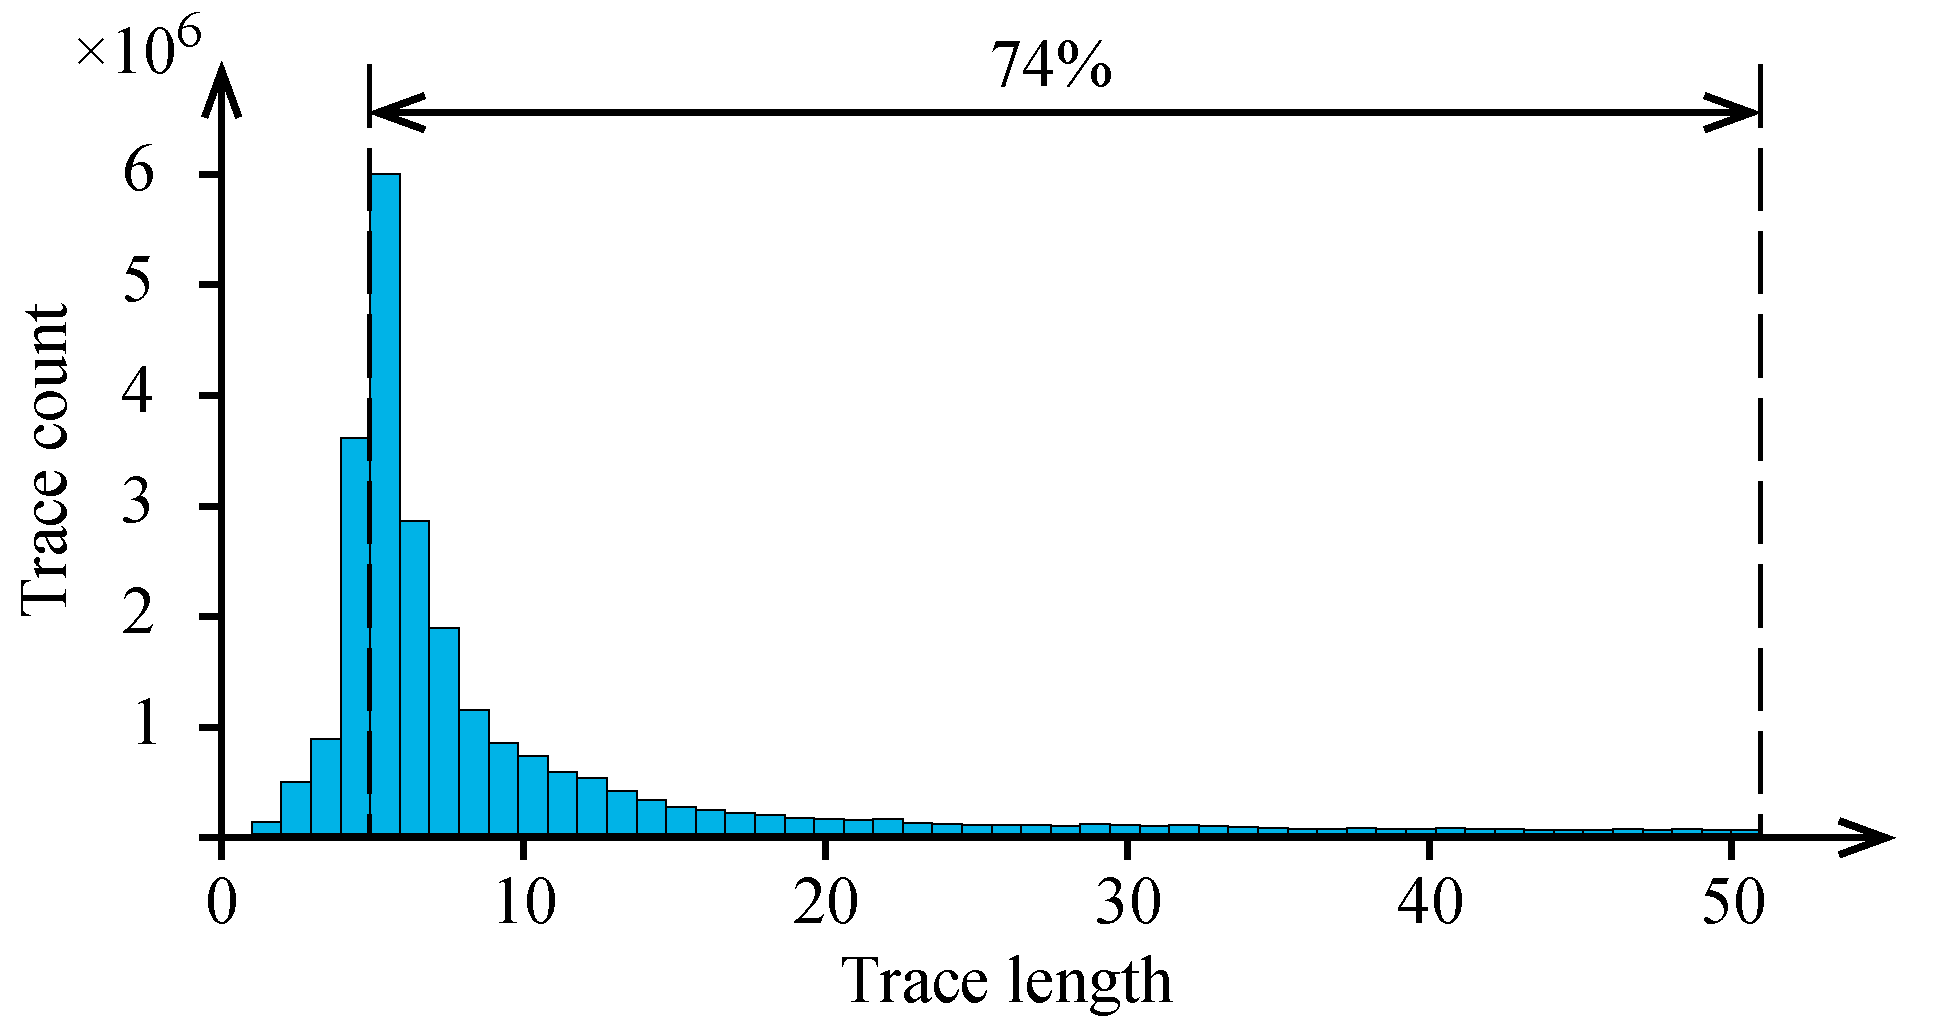
\includegraphics[width=1.0\columnwidth]{include/assets/figures/histogram.pdf}
  \caption{The histogram of the lengths of the resource-usage traces.}
  \flab{histogram}
\end{figure}

Regarding the selection stage delineated in \sref{selection}, we consider those
traces that contain 5--50 data points; in other words, we let $l_i \in [5, 50]$
in \eref{trace}. It can be seen in \fref{histogram}, which shows a truncated
histogram of the traces' lengths, that such traces constitute around 74\% of the
total number of traces (around 18 out of 24 million). The time taken by the
selection stage depends on the number of traces to be processed. For instance,
fetching and storing on disk one million random traces ($n = 10^6$ in
\eref{traces}) take less than three hours. This operation has to be repeated
only when the selection criteria change, which happens very rarely. We
considered two scenarios: $n = 10^6$ and $n = 2 \times 10^6$---which are roughly
5\% and 10\% of the 5--50 resource-usage traces, respectively---and,
consequently, the selection stage had to be done only twice.

\subsection{Modeling and Prediction}
She sells seashells on a seashore.
